\documentclass{acmsiggraph}
\usepackage{mathptmx}
\usepackage{graphicx}

\usepackage{parskip}

%%% short abstract
% By treating an image as a two-dimensional histogram, density-field
% data sets such as those created by chaotic maps can be visualized
% much more effectively and at interactive speeds.

\onlineid{poster\_0071}

\acmformat{print}

\title{Mapping Chaos (poster\_0071)}
\author{
  David Trowbridge\thanks{e-mail: trowbrds@cs.colorado.edu}
\and
  Micah Dowty\thanks{e-mail: micah@navi.cx}
}

\keywords{iterated function systems, chaotic maps, high dynamic range, animation}

\begin{document}

\maketitle

\section{Introduction}
\copyrightspace
Iterated Function Systems are a celebrated class of dynamical systems in the
computer graphics world. By defining a constrictive set of functions and
recursing, beautiful fractal images can be created. Classically, these
systems use a set of affine transformations, such as Sierpinski's Gasket.
More complex versions of these can be seen in the popular ``flame'' fractals
and single-orbit chaotic maps. When any of these systems is computed the
result is a density field which can then be rendered in any number of ways.

The traditional imaging techniques used to visualize these types of systems
are usually very simple, allowing only a few thousand points to be drawn.
However, with high-dynamic-range image processing techniques these images
can contain many millions of points, exposing far more internal structure.

\section{Exposition}
Generally the literature discussing chaotic maps and other systems which
produce density fields is full of greyscale images created where each pixel
is darkened as the point moves around the image region. This technique is
often sufficient for analyzing the structure of a map but does not provide
a sound basis for the use of the map as an artistic entity. The structure
of the attractor is only minimally visible using such techniques, because
a long iteration run will quickly result in a completely black image.

\begin{figure}[ht]
\centering
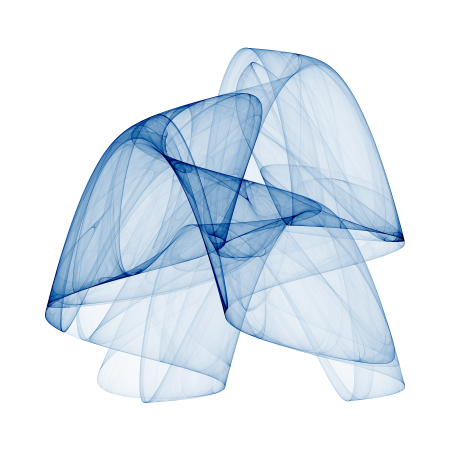
\includegraphics[width=2.5in]{1.png}
\caption{A complex attractor rendered as a two-dimensional histogram.
Fine details are made easily visible by color and shading. This image
contains approximately 100 million data points.}
\end{figure}

Instead, our technique treats the entire image region as a two dimensional
histogram. Unlike previous techniques, where each iteration is plotted by
darkening a a pixel directly, this histogram technique maintains total image
intensity as more iterations are performed. As more samples accumulate in the
histogram, the image simply gets more detailed. Instead of an image containing
only a few thousand iterations of the map, millions or billions of points can
be plotted with no loss of detail.

Like other rendering techniques that progressively refine an image, this
histogram method performes particularly well in interactive applications.
Our software for interactively browsing parameter space runs iterations
for each frame only until a predetermined amount of time has elapsed,
displaying a low quality but complete image nearly instantaneously.
Instead of waiting for a preset number of iterations to complete, the user
can zoom through parameter space quickly, viewing only what the CPU has time
to render. As soon as the user stops changing parameters, the image quality
will begin to improve.

Because a particular histogram bucket may contain tens of thousands of hits,
high-dynamic-range image processing techniques can be applied. This includes
gamma correction, exposure control, and color interpolation at the histogram's
full precision. By clamping each color component as late as possible in the
rendering process, the color can provide a visual hint at the higher
dynamic range of the image.

A histogram of infinitely small points can not be antialiased using standard
frequency filtering techniques, but aliasing artifacts can be reduced by
oversampling- using multiple histogram buckets per pixel.

\section{Conclusion}
Treating histograms as high-dynamic-range images creates the opportunity to
convey far more information in a single image than conventional techniques.
Simple greyscale images containing only a few thousand points can only begin
to hint at the true complexity of systems such as chaotic maps. This technique
is applicable to any large, geometrically constrained data set that can be
represented as a density field. It has shown to work particularly well in
the visualization of chaotic attractors and bifurcation diagrams of chaotic
systems.

The possibility of interactivity enables this technique to be used not only
for data visualization but as an artists tool. In particular, the ability
to interactively explore the parameter space of a chaotic map allows the
discovery of beautiful attractors which can then serve as textures or other
feed material. Possible future directions of this technique involve the use
of computer vision to automatically detect and avoid parameter sets which
result in non-chaotic attractors such as fixed points.

\end{document}
